% !TEX root = ../Thesis.tex
\myChapter{Computed Tomography}\label{ch:ct}
\begin{flushright}{\slshape    
		So Long, and Thanks for All the Fish!} \\ \medskip
    --- \defcitealias{Adams1984}{Douglas Adams}\citetalias{Adams1984} \citep{Adams1984}
\end{flushright}
\bigskip

\section{Computed Tomography}
Computed Tomography (\acs{CT}) has come a long way since its commercial availability in the late 1970, where Sir Godfrey Hounsfield invented the first commercially available thanks to the upcoming availability of microcomputers.

\begin{itemize}
    \item History
    \item Absorption -- Beer-Lambert
    \item Principles
    \begin{itemize}
        \item Sampling Theorem
        \item Reconstruction (FBP, gridrec)
    \end{itemize}
\end{itemize}

\section{The Swiss Light Source}

\renewcommand{\imsize}{0.618\linewidth}%
\begin{figure}[htb]
	\centering
	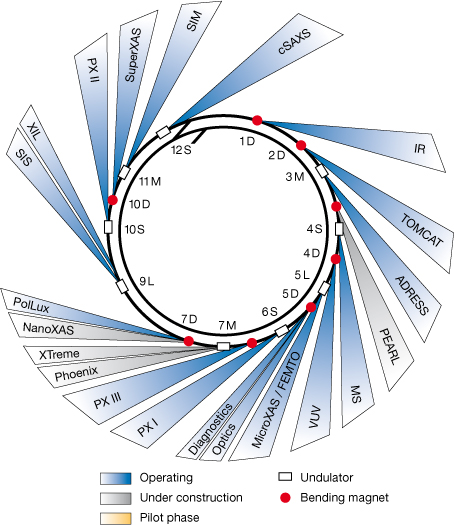
\includegraphics[width=\imsize]{img/SLS_beamlines_2008}
	\caption{Beamlines at the Swiss Light Source. Image from the \href{http://sls.web.psi.ch/view.php/beamlines/}{SLS Website}}
	\label{fig:beamlines}
\end{figure}

\section{TOMCAT}
A detailed explanation of the beamline for \acf{TOMCAT}, where all the tomography data for this thesis has been presented by \citet{Stampanoni2006a}.

As a short rundown the most important features of the beamline are presented here 

\renewcommand{\imsize}{0.5\linewidth}
\begin{figure}[htb]
	\subfloat[Overview of the Imaging Setup: The blue structure behind the control laptop is the sample stage. The black structure above contains the scintillator, the microscope optics and the camera.]{%
		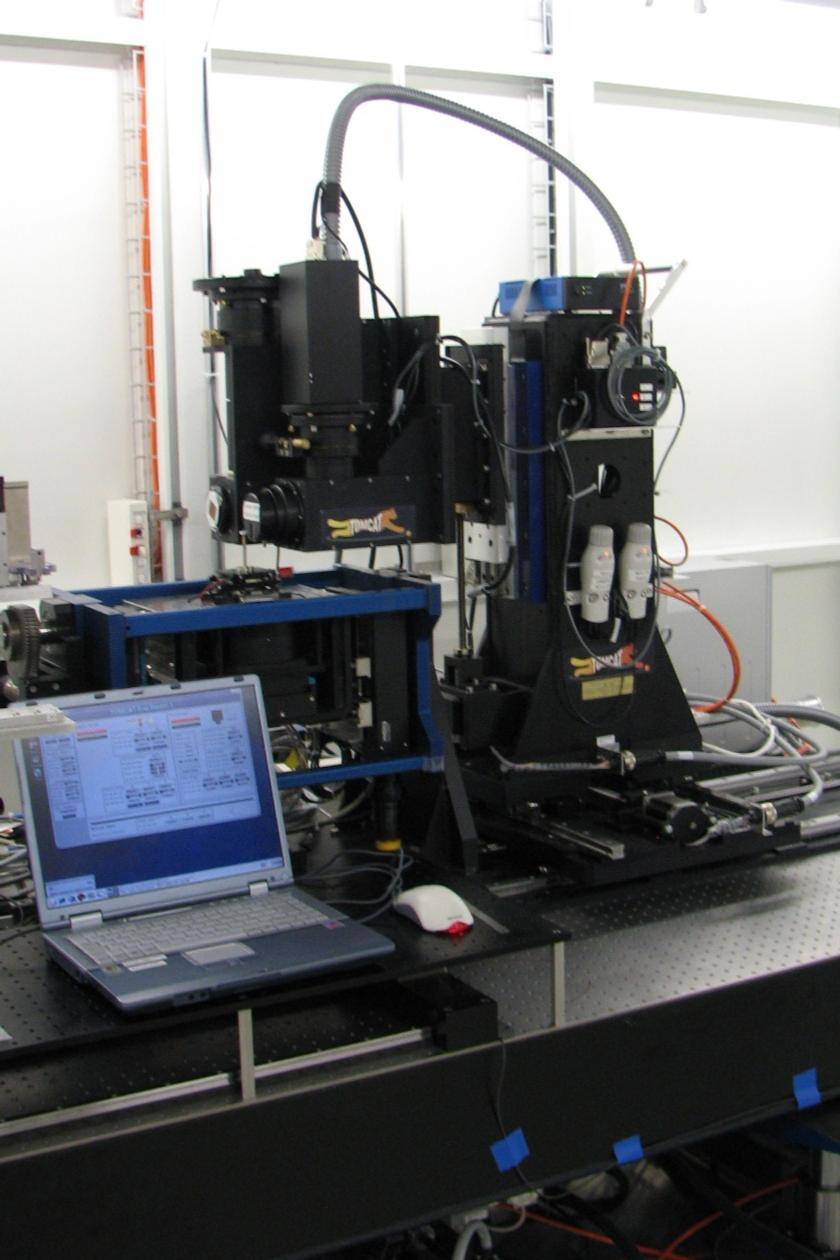
\includegraphics[width=\imsize]{img/TOMCAT1}%
		\label{subfig:TOMCAT1}%
		}%
	\subfloat[Close up view of a sample installed in front of the scintillator and microscope optics.]{%
		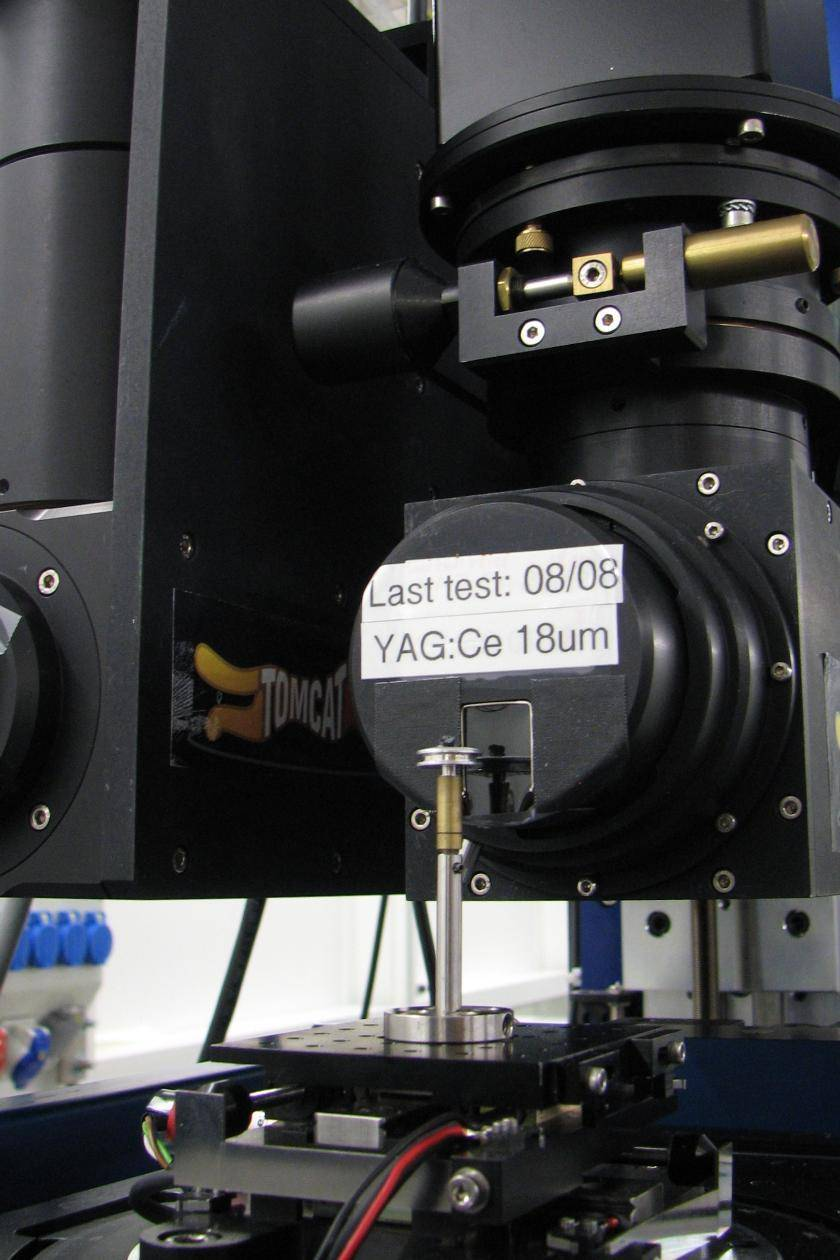
\includegraphics[width=\imsize]{img/TOMCAT2}%
		\label{subfig:TOMCAT2}%
		}%
	\caption{Images of the \ac{TOMCAT} beamline.}
\end{figure}

\begin{itemize}
    \item SLS
    \item TOMCAT
    \begin{itemize}
        \item Beam
        \item Sample Handling
        \item Data Acquisition
        \item Reconstruction
    \end{itemize}
\end{itemize}